%  A simple AAU report template.
%  2015-05-08 v. 1.2.0
%  Copyright 2010-2015 by Jesper Kjær Nielsen <jkn@es.aau.dk>
%
%  This is free software: you can redistribute it and/or modify
%  it under the terms of the GNU General Public License as published by
%  the Free Software Foundation, either version 3 of the License, or
%  (at your option) any later version.
%
%  This is distributed in the hope that it will be useful,
%  but WITHOUT ANY WARRANTY; without even the implied warranty of
%  MERCHANTABILITY or FITNESS FOR A PARTICULAR PURPOSE.  See the
%  GNU General Public License for more details.
%  TEST!
%  You can find the GNU General Public License at <http://www.gnu.org/licenses/>.
%
%  A simple AAU report template.
%  2015-05-08 v. 1.2.0
%  Copyright 2010-2015 by Jesper Kjær Nielsen <jkn@es.aau.dk>
%
%  This is free software: you can redistribute it and/or modify
%  it under the terms of the GNU General Public License as published by
%  the Free Software Foundation, either version 3 of the License, or
%  (at your option) any later version.
%
%  This is distributed in the hope that it will be useful,
%  but WITHOUT ANY WARRANTY; without even the implied warranty of
%  MERCHANTABILITY or FITNESS FOR A PARTICULAR PURPOSE.  See the
%  GNU General Public License for more details.
%
%  You can find the GNU General Public License at <http://www.gnu.org/licenses/>.
%
\documentclass[11pt,twoside,a4paper,openright]{report}
%%%%%%%%%%%%%%%%%%%%%%%%%%%%%%%%%%%%%%%%%%%%%%%%
% Language, Encoding and Fonts
% http://en.wikibooks.org/wiki/LaTeX/Internationalization
%%%%%%%%%%%%%%%%%%%%%%%%%%%%%%%%%%%%%%%%%%%%%%%%
% Select encoding of your inputs. Depends on
% your operating system and its default input
% encoding. Typically, you should use
%   Linux  : utf8 (most modern Linux distributions)
%            latin1 
%   Windows: ansinew
%            latin1 (works in most cases)
%   Mac    : applemac
% Notice that you can manually change the input
% encoding of your files by selecting "save as"
% an select the desired input encoding. 
\usepackage[utf8]{inputenc}
% Make latex understand and use the typographic
% rules of the language used in the document.
\usepackage[danish,english]{babel}
% Use the palatino font
\usepackage[sc]{mathpazo}
\linespread{1.05}         % Palatino needs more leading (space between lines)
% Choose the font encoding
\usepackage[T1]{fontenc}
%%%%%%%%%%%%%%%%%%%%%%%%%%%%%%%%%%%%%%%%%%%%%%%%
% Graphics and Tables
% http://en.wikibooks.org/wiki/LaTeX/Importing_Graphics
% http://en.wikibooks.org/wiki/LaTeX/Tables
% http://en.wikibooks.org/wiki/LaTeX/Colors
%%%%%%%%%%%%%%%%%%%%%%%%%%%%%%%%%%%%%%%%%%%%%%%%
% load a colour package
\usepackage{xcolor}
\definecolor{aaublue}{RGB}{33,26,82}% dark blue
% The standard graphics inclusion package
\usepackage{graphicx}
% Set up how figure and table captions are displayed
\usepackage{caption}
\captionsetup{%
  font=footnotesize,% set font size to footnotesize
  labelfont=bf % bold label (e.g., Figure 3.2) font
}
% Make the standard latex tables look so much better
\usepackage{array,booktabs}
% Enable the use of frames around, e.g., theorems
% The framed package is used in the example environment
\usepackage{framed}

%%%%%%%%%%%%%%%%%%%%%%%%%%%%%%%%%%%%%%%%%%%%%%%%
% Mathematics
% http://en.wikibooks.org/wiki/LaTeX/Mathematics
%%%%%%%%%%%%%%%%%%%%%%%%%%%%%%%%%%%%%%%%%%%%%%%%
% Defines new environments such as equation,
% align and split 
\usepackage{amsmath}
% Adds new math symbols
\usepackage{amssymb}
% Use theorems in your document
% The ntheorem package is also used for the example environment
% When using thmmarks, amsmath must be an option as well. Otherwise \eqref doesn't work anymore.
\usepackage[framed,amsmath,thmmarks]{ntheorem}

%%%%%%%%%%%%%%%%%%%%%%%%%%%%%%%%%%%%%%%%%%%%%%%%
% Page Layout
% http://en.wikibooks.org/wiki/LaTeX/Page_Layout
%%%%%%%%%%%%%%%%%%%%%%%%%%%%%%%%%%%%%%%%%%%%%%%%
% Change margins, papersize, etc of the document
\usepackage[
  inner=28mm,% left margin on an odd page
  outer=41mm,% right margin on an odd page
  ]{geometry}
% Modify how \chapter, \section, etc. look
% The titlesec package is very configureable
\usepackage{titlesec}
\titleformat{\chapter}[display]{\normalfont\huge\bfseries}{\chaptertitlename\ \thechapter}{20pt}{\Huge}
\titleformat*{\section}{\normalfont\Large\bfseries}
\titleformat*{\subsection}{\normalfont\large\bfseries}
\titleformat*{\subsubsection}{\normalfont\normalsize\bfseries}
%\titleformat*{\paragraph}{\normalfont\normalsize\bfseries}
%\titleformat*{\subparagraph}{\normalfont\normalsize\bfseries}

% Clear empty pages between chapters
\let\origdoublepage\cleardoublepage
\newcommand{\clearemptydoublepage}{%
  \clearpage
  {\pagestyle{empty}\origdoublepage}%
}
\let\cleardoublepage\clearemptydoublepage

% Change the headers and footers
\usepackage{fancyhdr}
\pagestyle{fancy}
\fancyhf{} %delete everything
\renewcommand{\headrulewidth}{0pt} %remove the horizontal line in the header
\fancyhead[RE]{\small\nouppercase\leftmark} %even page - chapter title
\fancyhead[LO]{\small\nouppercase\rightmark} %uneven page - section title
\fancyhead[LE,RO]{\thepage} %page number on all pages
% Do not stretch the content of a page. Instead,
% insert white space at the bottom of the page
\raggedbottom
% Enable arithmetics with length. Useful when
% typesetting the layout.
\usepackage{calc}

%%%%%%%%%%%%%%%%%%%%%%%%%%%%%%%%%%%%%%%%%%%%%%%%
% Bibliography
% http://en.wikibooks.org/wiki/LaTeX/Bibliography_Management
%%%%%%%%%%%%%%%%%%%%%%%%%%%%%%%%%%%%%%%%%%%%%%%%
\usepackage[backend=bibtex,
  bibencoding=utf8
  ]{biblatex}
\addbibresource{bib/mybib}

%%%%%%%%%%%%%%%%%%%%%%%%%%%%%%%%%%%%%%%%%%%%%%%%
% Misc
%%%%%%%%%%%%%%%%%%%%%%%%%%%%%%%%%%%%%%%%%%%%%%%%
% Add bibliography and index to the table of
% contents
\usepackage[nottoc]{tocbibind}
% Add the command \pageref{LastPage} which refers to the
% page number of the last page
\usepackage{lastpage}
% Add todo notes in the margin of the document
\usepackage[
%  disable, %turn off todonotes
  colorinlistoftodos, %enable a coloured square in the list of todos
  textwidth=\marginparwidth, %set the width of the todonotes
  textsize=scriptsize, %size of the text in the todonotes
  ]{todonotes}

%%%%%%%%%%%%%%%%%%%%%%%%%%%%%%%%%%%%%%%%%%%%%%%%
% Hyperlinks
% http://en.wikibooks.org/wiki/LaTeX/Hyperlinks
%%%%%%%%%%%%%%%%%%%%%%%%%%%%%%%%%%%%%%%%%%%%%%%%
% Enable hyperlinks and insert info into the pdf
% file. Hypperref should be loaded as one of the 
% last packages
\usepackage{hyperref}
\hypersetup{%
	pdfpagelabels=true,%
	plainpages=false,%
	pdfauthor={Author(s)},%
	pdftitle={Title},%
	pdfsubject={Subject},%
	bookmarksnumbered=true,%
	colorlinks=false,%
	citecolor=black,%
	filecolor=black,%
	linkcolor=black,% you should probably change this to black before printing
	urlcolor=black,%
	pdfstartview=FitH%
}
% package inclusion and set up of the document
%!TEX root = ../master.tex
% see, e.g., http://en.wikibooks.org/wiki/LaTeX/Formatting#Hyphenation
% for more information on word hyphenation
\hyphenation{ex-am-ple hy-phen-a-tion short}
\hyphenation{long la-tex}
% 
%!TEX root = ../master.tex
%  A simple AAU report template.
%  2015-05-08 v. 1.2.0
%  Copyright 2010-2015 by Jesper Kjær Nielsen <jkn@es.aau.dk>
%
%  This is free software: you can redistribute it and/or modify
%  it under the terms of the GNU General Public License as published by
%  the Free Software Foundation, either version 3 of the License, or
%  (at your option) any later version.
%
%  This is distributed in the hope that it will be useful,
%  but WITHOUT ANY WARRANTY; without even the implied warranty of
%  MERCHANTABILITY or FITNESS FOR A PARTICULAR PURPOSE.  See the
%  GNU General Public License for more details.
%
%  You can find the GNU General Public License at <http://www.gnu.org/licenses/>.
%
%
%
% see, e.g., http://en.wikibooks.org/wiki/LaTeX/Customizing_LaTeX#New_commands
% for more information on how to create macros

%%%%%%%%%%%%%%%%%%%%%%%%%%%%%%%%%%%%%%%%%%%%%%%%
% Macros for the titlepage
%%%%%%%%%%%%%%%%%%%%%%%%%%%%%%%%%%%%%%%%%%%%%%%%
%Creates the aau titlepage
\newcommand{\aautitlepage}[3]{%
  {
    %set up various length
    \ifx\titlepageleftcolumnwidth\undefined
      \newlength{\titlepageleftcolumnwidth}
      \newlength{\titlepagerightcolumnwidth}
    \fi
    \setlength{\titlepageleftcolumnwidth}{0.5\textwidth-\tabcolsep}
    \setlength{\titlepagerightcolumnwidth}{\textwidth-2\tabcolsep-\titlepageleftcolumnwidth}
    %create title page
    \thispagestyle{empty}
    \noindent%
    \begin{tabular}{@{}ll@{}}
      \parbox{\titlepageleftcolumnwidth}{
        \iflanguage{danish}{%
          
\includegraphics[width=\titlepageleftcolumnwidth]{figures/aau_logo_da}
        }{%
          
\includegraphics[width=\titlepageleftcolumnwidth]{figures/aau_logo_en}
        }
      } &
      \parbox{\titlepagerightcolumnwidth}{\raggedleft\sf\small
        #2
      }\bigskip\\
       #1 &
      \parbox[t]{\titlepagerightcolumnwidth}{%
      \textbf{Abstract:}\bigskip\par
        \fbox{\parbox{\titlepagerightcolumnwidth-2\fboxsep-2\fboxrule}{%
          #3
        }}
      }\\
    \end{tabular}
    \vfill
    \iflanguage{danish}{%
      \noindent{\footnotesize\emph{Rapportens indhold er frit tilgængeligt, men offentliggørelse (med kildeangivelse) må kun ske efter aftale med forfatterne.}}
    }
    \clearpage
  }
}

%Create english project info
\newcommand{\englishprojectinfo}[8]{%
  \parbox[t]{\titlepageleftcolumnwidth}{
    \textbf{Title:}\\ #1\bigskip\par
    \textbf{Theme:}\\ #2\bigskip\par
    \textbf{Project Period:}\\ #3\bigskip\par
    \textbf{Project Group:}\\ #4\bigskip\par
    \textbf{Participant(s):}\\ #5\bigskip\par
    \textbf{Supervisor(s):}\\ #6\bigskip\par
    \textbf{Copies:} #7\bigskip\par
    \textbf{Page Numbers:} 69 \bigskip\par
    \textbf{Date of Completion:}\\ #8
  }
}

%Create danish project info
\newcommand{\danishprojectinfo}[8]{%
  \parbox[t]{\titlepageleftcolumnwidth}{
    \textbf{Titel:}\\ #1\bigskip\par
    \textbf{Tema:}\\ #2\bigskip\par
    \textbf{Projektperiode:}\\ #3\bigskip\par
    \textbf{Projektgruppe:}\\ #4\bigskip\par
    \textbf{Deltager(e):}\\ #5\bigskip\par
    \textbf{Vejleder(e):}\\ #6\bigskip\par
    \textbf{Oplagstal:} #7\bigskip\par
    \textbf{Sidetal:} 69\bigskip\par
    \textbf{Afleveringsdato:}\\ #8
  }
}

%%%%%%%%%%%%%%%%%%%%%%%%%%%%%%%%%%%%%%%%%%%%%%%%
% An example environment
%%%%%%%%%%%%%%%%%%%%%%%%%%%%%%%%%%%%%%%%%%%%%%%%
\theoremheaderfont{\normalfont\bfseries}
\theorembodyfont{\normalfont}
\theoremstyle{break}
\def\theoremframecommand{{\color{gray!50}\vrule width 5pt \hspace{5pt}}}
\newshadedtheorem{exa}{Example}[chapter]
\newenvironment{example}[1]{%
		\begin{exa}[#1]
}{%
		\end{exa}
}
% my new macros

\begin{document}
%frontmatter
\pagestyle{empty} %disable headers and footers
\pagenumbering{roman} %use roman page numbering in the frontmatter
\graphicspath { {./figures/} }
%!TEX root = ../master.tex
%  A simple AAU report template.
%  2015-05-08 v. 1.2.0
%  Copyright 2010-2015 by Jesper Kjær Nielsen <jkn@es.aau.dk>
%
%  This is free software: you can redistribute it and/or modify
%  it under the terms of the GNU General Public License as published by
%  the Free Software Foundation, either version 3 of the License, or
%  (at your option) any later version.
%
%  This is distributed in the hope that it will be useful,
%  but WITHOUT ANY WARRANTY; without even the implied warranty of
%  MERCHANTABILITY or FITNESS FOR A PARTICULAR PURPOSE.  See the
%  GNU General Public License for more details.
%
%  You can find the GNU General Public License at <http://www.gnu.org/licenses/>.
%
\pdfbookmark[0]{Front page}{label:frontpage}%
\begin{titlepage}
  \addtolength{\hoffset}{0.5\evensidemargin-0.5\oddsidemargin} %set equal margins on the frontpage - remove this line if you want default margins
  \noindent%
  \begin{tabular}{@{}p{\textwidth}@{}}
    \toprule[2pt]
    \midrule
    \vspace{0.2cm}
    \begin{center}
    \Huge{\textbf{
      Report Title% insert your title here
    }}
    \end{center}
    \begin{center}
      \Large{
        - Subtitle -% insert your subtitle here
      }
    \end{center}
    \vspace{0.2cm}\\
    \midrule
    \toprule[2pt]
  \end{tabular}
  \vspace{4 cm}
  \begin{center}
    {\large
      Project Report%Insert document type (e.g., Project Report)
    }\\
    \vspace{0.2cm}
    {\Large
      MTA15341%Insert your group name or real names here
    }
  \end{center}
  \vfill
  \begin{center}
  Aalborg University\\
  Medialogy
  \end{center}
\end{titlepage}
\clearpage

\thispagestyle{empty}
{\small
\strut\vfill % push the content to the bottom of the page
\noindent Copyright \copyright{} Aalborg University 2015\par
\vspace{0.2cm}
\noindent{\footnotesize\emph{The content of this report is freely available, but publication (with reference) may only be pursued due to agreement with the author.}}
}
\clearpage


\pdfbookmark[0]{English title page}{label:titlepage_en}
\aautitlepage{%
  \englishprojectinfo{
    Augmented Boardgame %title
  }{%
    Visual Computing-Human Perception %theme
  }{%
    Autumn Semester 2015 %project period
  }{%
    MTA15341 % project group
  }{%
    %list of group members
    Daniel Vilcapaza\\ 
    Emilie Lind Damkjær\\
    Liv Arleth\\
    Markus Kristian Oerbæk Bertelsen\\
    Peter Kejser Jensen\\
    Rasmus Kaasgaard Christiansen
  }{%
    %list of supervisors
    Andreas Moegelmose
    
  }{%
    1 % number of printed copies
  }{%
    \today % date of completion
  }%
}{%department and address
  \textbf{Medialogy}\\
  Aalborg University\\
  \href{http://www.aau.dk}{http://www.aau.dk}
}{% the abstract
  Here is the abstract
}


\cleardoublepage
\pdfbookmark[0]{Contents}{label:contents}
\pagestyle{fancy} %enable headers and footers again
\tableofcontents
%\listoftodos
%\chapter*{Preface\markboth{Preface}{Preface}}\label{ch:preface}
\addcontentsline{toc}{chapter}{Preface}
Here is the preface. You should put your signatures at the end of the preface.

\vspace{\baselineskip}\hfill Aalborg University, \today
\vfill\noindent
\begin{minipage}[b]{0.45\textwidth}
 \centering
 \rule{\textwidth}{0.5pt}\\
  Author 1\\
 {\footnotesize <username1@XX.aau.dk>}
\end{minipage}
\hfill
\begin{minipage}[b]{0.45\textwidth}
 \centering
 \rule{\textwidth}{0.5pt}\\
  Author 2\\
 {\footnotesize <username2@XX.aau.dk>}
\end{minipage}
\vspace{3\baselineskip}
\begin{center}
\begin{minipage}[b]{0.45\textwidth}
 \centering
 \rule{\textwidth}{0.5pt}
  Author 3\\
 {\footnotesize <username3@XX.aau.dk>}
\end{minipage}
\end{center}

\cleardoublepage
%mainmatter
\pagenumbering{arabic} %use arabic page numbering in the mainmatter
%!TEX root = ../master.tex
\chapter{Introduction}\label{ch:introduction}

Board games come in many shapes, sizes, and levels of complexity. While some people see complexity as a pleasant challenge, others find it to be overwhelming, and therefore are these games intimidating to play. This is due to the players themselves are the only ones that can make sure that the game is being played according to the rules.

By incorporating computer-controlled elements into the board game, this project attempts to digitise and automate parts of it. This is to investigate, if a partly digitisation of the game can maintain the experience and enjoyment of play, while having certain parts handled by a computer.




\chapter{Initial Problem}\label{ch:ch2label}
Here we will explain our initial ideas and criteria we based our choices on.

We have based our initial problem formulation on our semester theme and our chosen project recommendation. Because of this, we wanted our initial problem formulation to be based on computer vision and a augmented board game, with the augmentation being based on computer vision. As we tried to specify what our analysis of the initial problem formulation should cover, we generated several ideas through brainstorming.

Those ideas each had a chosen board game, chosen technology needed for the ideas and a rough project process planning. Furthermore, all the ideas went through some criteria, in order to filter our ideas.
The criteria were:
\begin{enumerate}
	\item The idea must implement computer vision, since that is what we will need to fulfil our curriculum.
	\item The idea must include a existing board game that we have access to. So we do not design our own board game from scratch.
	\item The implemented computer vision for the idea must be interactive. This was important for us to remember, in order to stick with the main course of 3rd semester in the curriculum.
	\item The playtime of the idea's chosen board game must not have an average game time over two hours. This criteria was based on the assumption that if the game's playtime was too long, it would be harder to test it properly.
	\item The implemented computer vision may not make the board game itself more convoluted than it is. This criteria was added after a discussion, where the study group agreed on that we would not want to make the board games 'harder to play' than they were. ((maybe elaboration of rewording needed here).
\end{enumerate}

((Here there should be a list over our project ideas. I an not sure of what level of details are needed here, and how much of it should be in the appendix instead of this chapter - also, maybe there should even be a small detailed description of Terra mystica...not written by me))

The chosen project idea were a interactive board for the game Terra Mystica. We believed that such a project would require a projection of the board, while an implementation computer vision should detect physical game pieces on top of the board.
Our understanding of our chosen project idea lead us to make up an assumption of which things we would need to do in order to make our idea a reality:
\begin{enumerate}
\item First, we would need to make up the board for the projection. Here we imagined that the board's function and usability (project-wise)would be prioritised over cosmetics. We would then need to make the board a projection.
\item We then need the implemented computer vision to recognise the hexes that from a projected Terra Mystica board.
\item After that, the projected board must be able to change the colors of the hexes in it, since that is an essential visual part of the game itself.
\item The computer vision now needs to recognise the game pieces.
\item Now that the hexes can be recognised and change color while the game pieces also are being recognised, we will need to write/code(??!?) a program that can tie the hex color change to the game piece placement.
\end{enumerate}
%!TEX root = ../master.tex
\chapter{Background Research}\label{ch:bgres}
\todo{introduction to this chapter is needed. It needs an explanation to why this chapter is relevant}
The background research in this chapter is based on acquiring answers to the initial problem statement and the two research questions. The research includes studies of state of the art artefacts, previous work and which methods they used. 


\section{Target Group Explained}
The project's target group are people who are experienced with board games, maybe even Terra Mystica and are 14 years old or above since this is the game's recommended age group. This is because Terra Mystica itself caters to people who have a certain amount of experience with board games or people who like to play complex games, as the game has a lot of rules to keep track of. The project does not aim to simplify the game's core, but rather streamline the game mechanics, and therefore players who are inexperienced with complex board games will not benefit, since Terra Mystica is not a simple game to play.



\section{Previous scientific work}
In this section, other attempts to digitally augment board games will be discussed.

Andersen et al. \citep{andersen_designing_2004} created "BattleBoard3D", a board game utilising physical and digital components. For their physical components they used flat squares with patterns that through Augmented Reality (AR) technologies will be recognised through a camera and/or Virtual Reality goggles. Their research was made to illustrate "design issues for AR board games".

Peitz et al. \citep{peitzWizards2006} created "Wizard's Apprentice", a computer-augmented board game. The game includes two roles: wizard and apprentice. All players but one play as apprentices guided by the wizard who acts as a negotiator and motivator. The software is written in Java and has several play modes. The game uses Radio-Frequency Identification (RFID) hardware to detect at which physical point the players are in the game. It sends this information through antennas to a laptop close by. The laptop projects this information to a screen that displays relevant information on each player's turn. The game board can be seen in Figure \ref{fig:peitz}.

Magerkurth et al. \citep{magStars} created "STARS", a ubiquitous computing platform for computer augmented tabletop games. This platform includes devices such as a game table, a wall display, PDAs, and audio devices. The purpose of this platform was to provide features that went beyond what normal board games are capable of, while still maintaining the experience of the players interacting as they would with a normal board game. The platform was also able to save game states with ID tags, remember complex rules so they would not slow down the pacing of a game, and make the game board react dynamically to interactions with the game and its pieces. Its software is developer-friendly so that creating rules and content could be prioritised over device integration and game board management. 

\begin{figure}[!h]
\centering	
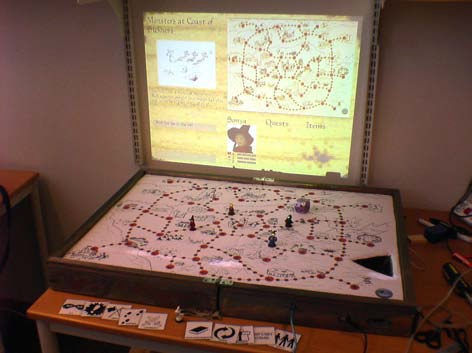
\includegraphics[width=0.5\textwidth]{peitz}
\caption{The Wizard's apprentice game board setup from \citep{peitzWizards2006}}
\label{fig:peitz}
\end{figure}

\section{Commercial competition}
Apart from previous scientific work, commercial board games have been released, existing on a spectrum ranging from completely digital to completely analogue. As our product will exist somewhere on the spectrum, these commercial solutions described below can be considered state of the art for this project.

\todo{do we need refs for these?}On the digital end, the online collectible card game Hearthstone (for Windows, OS X, Android and iOS), though completely virtual, has an interface which resembles a physical game board with cards and information on it. The user plays the game by dragging the cards onto the board from their 'hand' by way of using the cursor (when playing on a desktop computer), or by swiping with a finger (when playing on a smartphone or a tablet). The cards placed on the board can then be dragged to the cards they need to attack, etc. This swiping mechanism gives the game a tangible sense, making it resemble an analogue card game, even though no physical cards are involved.

There are also board games which integrate phone or tablet applications into the gameplay. One such game is XCOM: The Board Game, which simulates an alien attack the players then have to repel. The game has a physical game board, cards and pieces, but also a companion app, which can be downloaded to a desktop computer or mobile device. The app is required in order to play the game. It tracks the time each player has to do certain tasks, as well as what actions the aliens will take. The game therefore still looks like a normal board game, but it has a built-in augmentation in the form of the app, which changes the way turn/task orders and time constraints are done in a board game.

Another example of a board game which incorporates digital media is the card game, Munchkin. The game itself is a card game that can be played without augmentation. However, an app has been released which assists a player in keeping track of their current level and their combat strength compared to the monster they're fighting. Apart from that, the app provides the player using it with a bonus in the game. This is an example of a board game which has an optional digital augmentation, but it is not necessary to play the game.

\section{Methods for evaluating and measuring key success criteria}
Andersen et al. \citep{andersen_designing_2004} evaluated their product on a group of 13 year old children. The goals were to "reveal issues concerning the game design in general, design of the physical pieces, the use of goggles versus screen display, and future evolvement." The children found the 3D projection of the characters through the goggles fascinating, although some fumbling with the game pieces occurred due to the nature of the goggles and placement of the webcam. This occurred less when they looked at the 3D figures on the screen, but this brought along the problem of shifting focus away from the board game.
Finally, the children found the small set of animations uninteresting after a while and suggested a higher number of animations were needed to keep interest.

Peitz et al. \citep{peitzWizards2006} performed an initial evaluation on 3 children aged 8-9 and a male adult player (37). The evaluation was based upon a template that evaluates the social adaptability of game divided into: "(...)spatial, temporal, social, and playability." The participants were observed for two hours and were thematically interviewed afterwards. The participants reported overall enjoyment and increased togetherness in the game, but the pacing of the game felt unfamiliar. The participants seemed to particularly react positively to the sound design. 

\section{Competitive analysis}
As shown by Andersen et al. \citep{andersen_designing_2004}, a solution to enhance a board game can be done through AR aided by either a screen or Virtual Reality (VR) goggles. Andersen et al. mention some drawbacks to both of their technologies. In the case of AR with a screen they note that while the screen gives the participants the ability to look their opponent in the eye, they are distracted by having to look away from the board game space, to look at the screen displaying the figures. Regarding the VR, they note that participants liked the ability to pick up a game piece and explore all sides of the 3D model through the goggles. The problem, as can be seen in Figure \ref{fig:andersen}, could be that the goggles take away from the non-verbal communication that board games tend to foster.

In \citep{peitzWizards2006}, Peitz et al. built a board together with RFID antennas and other hardware to detect certain points of the the players' progression. They note some positive things, as aforementioned, namely the increased feeling of togetherness and overall enjoyment. They follow a recipe many traditional board games follow: a tile progression. They simulate this with the dots throughout the map, which the "tokens" press down on and activate. They also note the relationship between wizard and apprentices works well, but note an interesting development in the dynamics when one of the children effectively demotes the adult, who has the role as wizard, and temporarily acts as a new wizard. They did not account for this, but mention it is within their design goals.

As for the commercial competition, the solutions utilise digital media to varying degrees, in some cases combining these elements with traditional board game elements such as a board or cards, bringing in the aforementioned feeling of togetherness identified by Peitz et al \citep{peitzWizards2006}. However, in these multi-media solutions, the digital aspects are not integrated physically into the game, but rather exist as additional, separate 'piece' of the game in the form of a phone, tablet for personal computer. There is an unutilised potential in combining digital and physical elements in such a way that the players can feel the unity board games provide without the barrier of a screen between them, but at the same time have a program handle some of the management of parts, reducing the amount of time players have to spend on that.

\begin{figure}[!h]
\centering	
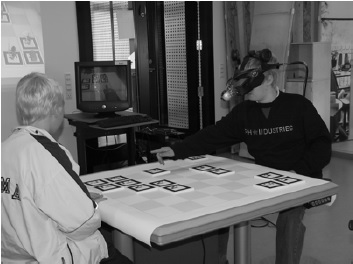
\includegraphics[width=0.5\textwidth]{andersen}
\caption{BattleBoard3D setup from Andersen et al.  \citep{andersen_designing_2004}}
\label{fig:andersen}
\end{figure}


\section{Terra Mystica}
Terra Mystica is a game that utilise a lot of different game pieces for different tasks. One of the tasks that use a lot of pieces is the task of terraforming a terrain into the factions home terrain. In some games a player can terraform so much that he/she runs out of pieces to terraform with. This problem could be solved though an interactive board, that removes the terrain pieces, and instead just changes the board itself. This way there is no way to run out of terraforming pieces.

\textbf{Power}

A mechanic often forgotten in the game is that when you build next to another player, you have to offer that player a thing called power, based on which building are adjacent to the build you just placed, and if the power value is above one, you lose victory points based on power value minus one. With an augmentation it would be possible for the game to tell the players involved in the offering of power, to just get a notice that tells them exactly how much power they would gain, and how many victory points they would lose on it.

\textbf{Cult track}

Terra Mystica has a mechanic called the cult track, which is a separate board with four different cults on it, as the game progresses players may gain cult points which grants them power, and in the end of the game, the players with the highest,second highest, and third highest value in the cult track gains additional points based on their position. Through an augmentation to the game it would be possible to make the cult track a program, that kept track of who was where, and who was winning the different tracks. 
%!TEX root = ../master.tex
\chapter{Final Problem}\label{ch:finprob}
The initial problem formulation provided research questions to expand our understanding of the problem area. The following final problem formulation is instead focused on the development of our product.

\section{Formulation}
After having chosen Terra Mystica as the board game to augment, the augmentation was decided as being an interactive game board via computer vision.

The initial research questions were:
\begin{itemize}
	\item How can computer vision be used to facilitate user interaction?
	\item How should the software for that be developed?
\end{itemize}

As seen in previous scientific work with examples of current state of the art, Andersen et al. \citep{andersen_designing_2004} used recognition technology via camera and Peitz et al. \citep{peitzWizards2006} showed the output from a game unto a projection. Both can add inspiration to how the initial research questions may be answered. An example being, creating an interactive projection, and having it being manipulated through interaction with its computer vision software.

The results of the ensuing background research were that BLOB recognition and background imaging in an RID solution would be a possible facilitation.
The software for that should be designed in such a way that the user can:
\begin{itemize}
\item Control the turn order
\item Start and end their own turn
\item Change a tile on the screen by 'terraforming'
\end{itemize}

In this project, an unutilised potential was identified when researching how augmentation like the current project idea would affect the usability of the game, in comparison to the non-augmented version. All that culminates into the final problem formulation:

\textit{“Can Terra Mystica become more usable through the use of a computer vision augmented board?”}

\subsection{Success Criteria}
\todo{this description seems vague, I might fix it later, else I am open for ideas}\todo{I did something new - Liv}
When defining the problem for the project, certain criteria were defined that needs to be met if the project is to be deemed a success. The success criteria have been defined as following:

\begin{itemize}
	\item The projection software must be able to make the image of the board game show one of seven different tiles in each interactive tile, and make tiles changeable, in order to make the user able to do terraforming in the game.
	\item The augmented game board must be usable for a whole game, so that the augmented version of Terra Mystica could replace the unaugmented one. That also means a game of Terra Mystica should not be halted or stopped by any technical problems.
	\item The computer vision software needs to register some sort of BLOB, in order to make the board game change the tiles. This means an implementation image processing that works with the projection of the board.
\end{itemize} \todo{maybe more can be added, but I don't know what}
=======

 
%!TEX root = ../master.tex
\chapter{Development}\label{ch:development}
Our development chapter. \todo{We describe Rear Infused Illumination, and add all theory we have on the things mention if RID - for example BLOBs, contrast, illumination and so on }

\section{Rear Diffused Illumination}
The interaction on our game board table will be based on rear diffused illumination as described in Multi-Touch Technologies\citep{multiTT}. As shown in figure ((ref project sketch)) this means we are going to make inputs in the augmented board game via having it recognise the touch of the board as BLOBs shown in IR light. This is because of a camera beneath the table's surface that observes a change in the contrast shown in IR light. 
For this to work, a table's top surface, made of transparent material, needs a diffusermaterial just above or beneath it in order to diffuse the light. Infra-red light then needs to be shined on it from beneath the surface. When the glass is pressed from above the surface by an object, that part of the surface reflects more light back which will be captured by the camera as a BLOB.

\begin{figure}[!h]
\centering	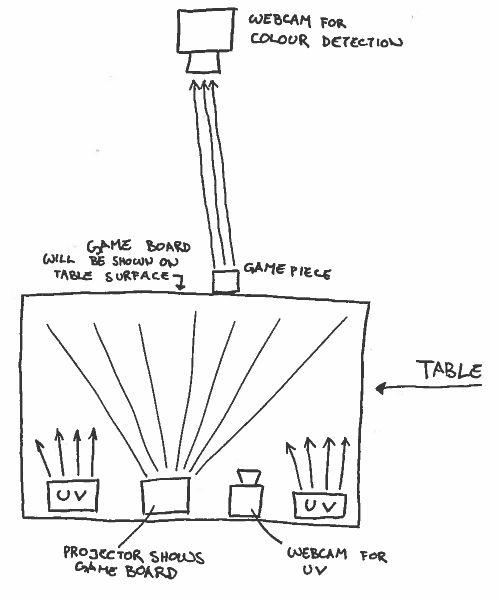
\includegraphics[width=0.5\textwidth]{TouchBoardDiagramSketch}
\end{figure}

Choosing such a solution has it's advantages and disadvantages. First of all, there is no need for a compliant surface or soldering for a LED frame, since we are using a diffuser in order to reflect the IR-light coming from below. The illuminators for that can be bought ready to go, so there is no need to build them. A disadvantage comes from the RDI having difficulties with getting even illumination, since the IR-lights might cover the table's surface completely. This can result in false BLOBs and BLOBs of lower contrast, which will challenge the software's detection of the real BLOBs.

\section{Physical Design} 
This section will describe the physical aspect of our product.
We have assembled a touch board, made with a plexi glass top and IR lamps below. Underneath the surface of the top is a short throw projector so we are able to project images on the table. Additionally we have a web camera on the very bottom of the table to be able to detect, via the IR lamps any changes, in form of touches or placed game pieces, in the surface of the board. 
The field of view of the camera is 74cm*58cm, and the entire table top is 102cm*120cm. The table is 95cm. 
a

\section{Technology}


%!TEX root = ../master.tex
\chapter{Final Prototype}\label{ch:finproduct}
The following chapter contains a description of the state of the prototype, at the end of the project period.

\section{Physical prototype}
The table is constructed by aluminium extrusions, measuring 120 x 102 x 89 cm. A shelf is located on the internal side of the top frame, which is used to hold a 3 mm acrylic glass plate. The underside of the glass is covered in a single layer of baking paper. This acts as the diffusion material in the RDI setup, as well as the screen for the short-throw projector.

In the bottom of the table are extrusions, which hold the rest of the RDI setup and the projector. The camera is placed at the bottom of the table, so that the area of sight is larger. The projector is placed to one side of the table, as this makes the cone of projection land centrally on the screen. The IR lights are placed 30 cm into the air, by mounting them on top of extrusions. This height is optimal, as the camera can detect more, the closer the lamps are to the screen. However, the closer the lamps are to the screen, the smaller the cones are of infra-red light.  Furthermore, if the lamps were to be placed higher, the extrusions they were mounted on would then start blocking the projector, making parts of the screen not viewable by the users. In order to contain the IR light inside the table, a black cloth baffle is placed around the sides of the table.

A computer runs the software and is connected to the camera and projector. The camera acts as input for the software, and the projector shows the output on the screen.

\section{Digital prototype}
The prototype displays a recreation of the Terra Mystica board and includes the following graphics:
\begin{itemize}
	\item The hexagonal tiles in the seven different colours, plus the river tiles
	\item An inner frame around the board tiles, which is used to track each player's amount of victory points.
	\item An outer frame, which contains a table with instructions on how to score victory points at the end of each round and at the end of the game. It also contains an undo button and buttons for actions that can be taken by only one player each round.
\end{itemize}

\subsection{Interactive elements}
The tiles are interactive, as the game's primary interaction with the board is terraforming. Each tile is independently interacted with, and can be changed to the colour of the current player, using hand gestures. In the original game, it costs different amounts of resources to change different colours, depending on the colour of the player. The table does not manage this, and relies on the players managing the resources required themselves.

When a player starts their turn, they must make a gesture, so the system knows which colour to use if the player wants to terraform. Since the low amount of lamps used cause the middle area of the board to be more illuminated, and thus more responsive, than the outer edges, these gestures are done in the middle, as opposed to in the designated areas, as per the original design. In order to make the player selection more reliable, paper hands are given to each player to be used instead of their actual hands.

\subsection{Non-interactive elements}
The victory point tracker is not an interactive piece of the board. Instead, it is a static graphic, where each player has a game piece placed on their current number of victory points.

The outer frame also includes two undo buttons, placed in opposite corners, which was meant to give the players the ability to revert the last action taken. However, this is not implemented because of time constraints.

In the two other corners, an area displaying  the goals is placed. This is described with images illustrating what players will get victory points for in each round. Images illustrating what players score victory points for in the end of the game are also in this area. In the original game, this table can have random objectives for each round, but in the digital version, it is a static image used as a place holder.
%!TEX root = ../master.tex
\chapter{Code Overview}\label{ch:codeover}

\section{Point-processing}
There are three point-processing algorithms in this software; an RGB-to-Greyscale colour conversion algorithm, a normalization algorithm, and a thresholding algorithm. All of these make use of double-nested \texttt{for}-loops to apply their operations to each pixel as shown in Figure~\ref{fig:pointprocess}.
\begin{figure}[!h]
\begin{lstlisting}
for (int y = 0; y < src.rows; ++y)
{
	for (int x = 0; x < src.cols; ++x)
	{
		//Code here...
	}
}
\end{lstlisting}
\caption{Basic point-processing algorithm. \label{fig:pointprocess}}
\end{figure} 

The RGB-to-Greyscale algorithm creates an 8-bit single-channel image and then maps the mean of the RGB-values of the input image pixels to the output like shown in Figure~\ref{fig:rgb2gray}

\begin{figure}[!h]
\begin{lstlisting}
output.at<uchar>(y, x) = (src.at<Vec3b>(y, x)[0] + src.at<Vec3b>(y, x)[1] + src.at<Vec3b>(y, x)[2]) / 3;
\end{lstlisting}
\caption{RGB-to-Greyscale operation.\label{fig:rgb2gray}}
\end{figure}

The normalization algorithm finds the maximum and minimum pixel values of the input image using an OpenCV function. It then processes each pixel to normalize them to a new maximum and minimum using the operation shown in Figure~\ref{fig:normalize}.

\begin{figure}
\begin{lstlisting}
output.at<uchar>(y, x) = floor((src.at<uchar>(y, x) - min) * (newMax - newMin) / (max - min) + newMin);
\end{lstlisting}
\caption{Normalization of a pixel. \label{fig:normalize}}
\end{figure} 

Finally, the thresholding algorithm determines whether a given output pixel is white or black based on the if-else statement that is shown in Figure~\ref{fig:threshold}.

\begin{figure}
\begin{lstlisting}
if (src.at<uchar>(y, x) >= threshold)
{
	src.at<uchar>(y, x) = 255;
}
else
{
	src.at<uchar>(y, x) = 0;
}
\end{lstlisting}
\caption{Thresholding. If the pixel value is above the threshold, make it white. Else, make it black.\label{fig:threshold}}
\end{figure}

\section{BLOB extraction}
After segmentation, a grass-fire implementation scans the image for BLOBs. First, a nested \texttt{for}-loop like the one shown in Figure~\ref{fig:pointprocess} goes through every pixel to check whether any of them is white (i.e. part of the foreground). If this condition is met, the function will call another function, which contains the actual grass-fire algorithm. The grass-fire function is called with the position of the white pixel and the image itself as arguments. 
%!TEX root = ../master.tex
\chapter{Testing and Evaluation}\label{ch:testeval}
In order to evaluate the product and see to what extent it can be considered successful, a usability test will be conducted.

\section{Purpose of test}
The purpose of this test is to test usability and functionality of the product. The ISO 9241 \citep{ISO} standard defines usability as effectiveness, efficiency, and satisfaction of the user. Put more precisely, this means:
\begin{itemize}
\item Efectiveness: To what extent are the goals of the product achieved?
\item Efficiency: What resources (including time) are expended to achieve the goals?
\item Satisfaction: To what extent does the user find the system acceptable?
\end{itemize}
With these in mind, the test aims to clarify whether the product lives up to its test objectives.

\section{Test objectives}
Our problem statement is defined in Section~\ref{sec:ProblemStatement}. Based on this problem statement, it is important not only to test how well the program functions on a technical level, but also if the test participants still feel like they are playing the original board game, which will be tested on a level of satisfaction/acceptance.
The success criteria (Section~\ref{sec:SuccessCriteria}) and the system requirements (Section~\ref{sec:ReqSpec}) each add to the specifications on the technical and satisfactory  objectives of the test.
These parts together make up these test objectives:

\begin{enumerate}
\item Do the players still feel like they are playing Terra Mystica, when they are playing the augmented version? \todo{this might need specifications or a broader question}
\item Do the players feel like taking turns using the player selection gestures is an easy task, or a hindrance?
\item How well are players able to undo mistakes they did while terraforming?
\begin{enumerate}
\item Furthermore, does the player selection task live up to the requirement specification that it should be successful 90\% of the time?
\end{enumerate}
\item Do the players feel like the task of terraforming is easier to carry out than on the original board game?
\begin{enumerate}
\item Furthermore, does the terraforming task live up to the requirement specification that it should be successful 75\% of the time?
\end{enumerate}
\item How easily are players able to undo mistakes they did while terraforming?
\begin{enumerate}
\item Furthermore, does the undo task live up to the requirement specification that it should be successful 50\% of the time?
\end{enumerate}
\item Do the players feel that the augmented game board can replace the original game board?
\item How hindered is the pace of the game by the three actions each player can take (chose player, terraform and undo)?
\end{enumerate}

These objectives set the goals for the test, and help determine whether or not the test is successful. 

\section{Test methods}
The test methods used, their criteria and their measurement are meant to see if the test objectives are met.

\subsection{Test set-up}
The test will take place in a controlled setting, were nobody else than the test participants and testers will be present around the board while a game is taking place. The participants will be playing, and the testers will only act as observers who document the proceedings, and helpers/guides - in case the participants have any technical problems that prevent them from proceeding from the test.
The documentation of the test will be done by a tester filming the participants playing the game and a note-taker that also acts as the spokesperson for the testers.

\subsection{Participants}
The chosen test participants are typical users. They are within the target group, which is defined in Section~\ref{sec:TargetGroup}, meaning that they are experienced with board games. \todo{Write some more stuff when participants are selected}

\subsection{Procedure}
The test, when set up, will follow this procedure:

\begin{enumerate}
\item To begin with, the test guide will introduce the participants to the product, and explain the whole test procedure. The guide will have a script to read from, to make sure all participants are fully informed.
\item Once all participants understand the procedure, they will begin a game of Terra Mystica using the augmented board\todo{how long? we'll find out in pilot test}. During the introduction, they are encouraged to have dialogues with each other regarding their actions and thoughts as they play. This is inspired by the think aloud method addressed by Larsen \citep{TestingLecture}. The whole test is filmed by the cameraman. It is especially imortant to get footage of the participants' hands as they attempt to do gestures. It is likely that all of the typical tasks will be performed during this playthrough, but if not, the test guide will ask the test participants to attempt the ones they forewent.
\item Once the practical part of the test is over, the test guide will conduct a semi-structured group \todo{depending on amount of testers} interview, which the participants have been informed about during the introduction. The participants will be asked about how they experienced the augmented game, both in its own right, and in comparison to the original game.
\end{enumerate}

Once the test is done, the footage and notes from the test will be analysed and compared to the test objectives.

\section{Results}
text\todo{analysis and conclusion}\todo{remember to look at video to analyse delay of actions and how many tries before successful action}
%!TEX root = ../master.tex
\chapter{Further Implementations}\label{ch:furthimp}
Hurdy dur intro\todo{we need an intro here}\todo{this whole chapter will be reiterated after evaluation}

\section{Additional functions}
Further implementation is possible in the functions of the augmented board game. Although we had originally planned to implement an undo button, it is not a part of the current version. If that function should have been included, it should have been an interactive area of interest separate from the map. This area should also be a visible part of the board’s GUI. An algorithm for this function could be a stacking system that remembers previous actions, allowing the program to revert them, returning to previous states of the program.

Another additional function to include could be for each player to choose their own faction from the game. Also, one should be able to add a colour to that faction, so it would display the chosen colour on the board when it was the faction’s turn. When a faction is selected, its counterpart (the backside of a faction’s card), should be inaccessible.

Lastly, the global power actions mentioned in Section \ref{sec:BoardInterface} could be an interactive function instead of spaces that you put game pieces on. The idea is to make the players able to press the powers, which would then make the powers become inaccessible. An advanced version of this function could have the program register faction rules, which would make the global actions still accessible to them. 

\section{Player assistance}
In order to assist players and streamline the game pace, the following further implementations could be done.

The program could remember which players have placed their buildings on each tile. When a player places or upgrades a building next to a tile which is occupied by another player, the game could remind one player to offer the other power. Ideally, even the specific type of building already occupying the surrounding tiles is remembered by the program, allowing it to calculate exactly how much power is to be offered to a player.

As of now, the interface has the global goals for each round displayed, but they are fixed, as opposed to randomised like in the original game. A possible iteration for this is to make the program draw randomised one-round goals in the beginning of the game, keeping each game unique. Goals for previous rounds that are no longer relevant could be hidden.

Another possible iteration is to make the colour of the currently selected player visible on the board, perhaps in the form of a border around the board. This way, players will not be in doubt whether or not they have correctly selected a player.

To assist the player with the management of their points during and at the end of the game, a feature which does the point registration and mathematical tasks could be added. In order for this to work, some subtraction and addition in a player’s amount of points should happen due what happens in the game and what the state of the game is at its end. Examples of such scenarios are: when a player receives power that would make them lose points, when a player reaches specific goals in the game, when a player places a specific building, etc. 

In the original game, each player has a card containing all information about their chosen race. This card could be made digital. This would open up the opportunity for players to ask the game for tips about specific icons and what they mean, in case they fail to remember.

Furthermore, the card keeping track of how many points each player has with each cult could be made digital. This digital board could react when players pass the given milestones on the track, reminding them to receive power. If this and the aspect overseeing goals are both implemented, the cult track could even award the players with the correct one-round bonuses currently in effect.  

\section{Technical tweaks}
As the original game can be played by 2-5 players, an ideal iteration of the program is to widen its capacity to 5 players. For a more advanced implementation, the board's GUI could change, due to the numbers of players in the game.

To achieve more precise BLOBs and make the program respond better to user input, a background subtraction step can be added to the segmentation process.
%!TEX root = ../master.tex
\chapter{Conclusion}\label{ch:conclusion}
Based on the results from the testing and evaluation of the prototype for the augmented Terra Mystica board, both usability-wise and technologically (Chapter \ref{ch:testeval}), an answer can be given to the problem statement from Section \ref{sec:ProblemStatement}.

\section{Problem Formulation}
The problem formulation is twofold:

\textit{“Can Terra Mystica become more usable through the use of a computer vision augmented board…”}

According to the results from this project, the answer is \textit{not at the prototype’s current state, but possibly in the future}. When testing the prototype, it became clear from the participants' usage that it slowed down the pace of the game because functions were not working efficiently. It was the terraforming and turn mechanics that took longer than in the original version of the game, which was caused by the users having trouble doing those actions. Despite this, some of the participants said they expected the actions not to be an hindrance at all if their functionality worked flawlessly. Some participants expected a faster pace of the game, if the augmented version had functions which took care of a player’s resource management. Furthermore, participants saw a potential in the augmentation interface design, since they believed its simplistic design would benefit new players, and that it could have a more explanatory GUI, which for the new players might increase the game’s usability. All this will require an improved version of the prototype. It should then be tested in order to see if those ideas do increase the game’s usability. This is why, may only in a later version make Terra Mystica become more usable through the use of a computer vision augmented board.\\
\\

\textit{“...while still maintaining the feeling of playing a traditional board game?”}

With the results in mind, the answer here is \textit{the prototype kept the players feeling like they still were playing a traditional board game, although the augmentation could change the game’s purpose}. The consensus between the participants was that they felt like they were playing the same game in both versions, despite the difference in how some actions in the game were executed. However, there were still participants who saw another change in the game’s purpose from the original to the augmented one. Some saw the augmented version as a simpler, larger, and clearer version of the two. Others saw the augmented board game as a more dramatic game to play, since instead of placing tokens for terraforming, you used your hands to do it. Additionally, some saw the two versions of the games as two ways of playing it, since one was by a large box you had to stand up to use, while light was shining from the board, and the other was a smaller, more tactile version, were you sat down and were closer to each other. In conclusion, the participants still felt like they were playing Terra Mystica, and it maintained the board game feeling, even though the different versions could represent different purposes of use.

\section{Success Criteria}
\textit{"The project must have gone through evaluations and iterations, based on relevant usability principles."}

The prototype was developed through multiple stages, first being tested as a paper mock-up. After this initial lo-fi testing, the feedback led to the second stage of development, which made use of the RDI setup for the use of terraforming. This stage was then tested with more participants, whose feedback led to establishing steps for further implementations of the augmented board game.\\
\\

\textit{"Augmentation technology must be utilised with Terra Mystica in such a way that it does not take away from the experience of the game but enhances it."}

In the usability testing of the prototype, many participants expressed positive interest in the board, when asked how they would respond if the prototype was developed into a fully implemented product. However, when asked if the prototype could replace the board game in its current state, the participants answered much more negatively, as technical issues and difficulties with RDI slowed the game’s pace and made hand gesture detection unreliable. Although some players reported that the simpler graphics of the augmented board was easier to get an overview from, others said the same from the more detailed tiles of the original board. Therefore, this success criterion is not fulfilled, with the prototype in its current state.\\
\\

\textit{"Implemented augmentation technologies should utilise computer vision to augment Terra Mystica"}

By making use of an RDI setup in order to detect gestures in the augmentation, the prototype removed the use of cardboard disks when terraforming. Instead it makes use of the player placing their hand on the table, in order to terraform and change turns. Therefore, this success criterion is fulfilled.\\
\\

\textit{"The accuracy and effectiveness of the image detection should be tested in a proper framework."}

The image detection implemented in the prototype was tested according to the framework described in Section \ref{subsec:techtest}, where accuracy, effectiveness, and overall efficiency of the system are tested. Appendix~\ref{app:techTest} documents the results of the testing carried out. However, whether it is a proper framework is debatable, as it is not built upon previous known methods of technical testing. Nonetheless, because of its defined procedural structure and clear display of data, this success criterion is considered to be fulfilled.
\bibliography{bib/mybib}
\label{bib:mybiblio}
\appendix
%!TEX root = ../master.tex
\chapter{Evaluation script}\label{ch:TestScript}
\section{Introduction to test}
(To the whole group)
Hello, and thank you all for agreeing to participate in our test. We have created a touch board table on which you can play the board game Terra Mystica. In other words, our product is a digitally augmented version of Terra Mystica.

You will start out by playing three rounds of the game on the [digital/analogue] version. While you play, you are encouraged to talk amongst each other about the game, and voice your thoughts. Once the three rounds are up, we will switch to the [digital/analogue] version, on which you will also play three rounds.

When you have played the two games, we will hold a short interview where you will be asked questions about your thoughts towards the augmented game. In this interview, you will also be asked to compare this version to the original game.

\section{Introduction to Terra Mystica rules}
For the purpose of this test, you will play a simplified version of the game.


\section{Explanation of the analogue version}
[Assuming they have played the digital version first]
The analogue version is played the same as the digital version, except you do not do a gesture when taking your turn, and you terraform by placing a token of your own colour on the tile you wish to terraform, like this [show it]. The buildings you wish to place are place on top of this token, like this [show it].

\section{Explanation of the digital version}
[Assuming they have played the analogue version first]
The digital version is played the same as the analogue version, except you now need to register yourself every time it is your turn, like this [show it], and instead of placing the tile tokens, you instead terraform like this[show it]. You will still place the buildings like before [show it].

\section{Post-test interview}
The following are points which needs coverage. This means that they should be used for a semistructured interview (meaning that the interviewer can, at any time, ask the interviewee to elaborate), made up by the questions raised from the testing and from the following: 
\begin{itemize}
\item How did you think the augmented Terra Mystica compares to the original game?
\begin{itemize}
\item Do you still feel like you were playing the same game when you were playing the augmented version?
\end{itemize}
\item How did you experience the act of indicating that is was your turn? Did you experience it as easy or difficult?
\begin{itemize}
\item How is the experience of taking turns in comparison to when playing the original game?
\end{itemize}
\item Did you experience ease or difficulty when terraforming compared to the original game?
\item Do you think the augmented game can serve as a possible replacement for the original board?
\item How do you think the game's pace was affected by the augmentation? Do you think it was increased or decreased?
\end{itemize}



\end{document}
